\chapter{Differential Equations}

Differential equations are equations involving an unknown function and
its derivatives. They play a crucial role in mathematics, physics,
engineering, economics, and other disciplines due to their ability to
describe change over time or in response to changing conditions.\index{differential equations}

\section{Ordinary Differential Equations}

An ordinary differential equation (ODE) involves a function of a
single independent variable and its derivatives. The order of an ODE
is determined by the order of the highest derivative present in the
equation. An example of a first-order ODE is:\index{ordinary
  differential equation} \index{ODEs}

\begin{equation}
\frac{dy}{dx} + y = x
\end{equation}

Here, $y$ is the function of the independent variable $x$, and 
$\frac{dy}{dx}$ represents its first derivative.

\subsection{Separable Differential Equations}
Sometimes, differential equations can be explicitly solved. A 
first-order differential equation is separable if $\frac{dy}{dx}$ can 
be written as a function of $x$ times a function of $y$. Symbolically, 
a differential equation is separable if it takes the form 
$$\frac{dy}{dx} = g(x)f(y)$$

The equations may be solvable by separating the $x$ from the $y$ and 
integrating each side. For our generic form, we can separate the 
variables thusly if $f(y) \neq 0$: 
$$\frac{dy}{dx}\frac{1}{f(y)} = g(x)$$ 
$$\frac{1}{f(y)}dy = g(x) dx$$ \\
Integrating both sides: $$\int \frac{1}{f(y)}\,dy = \int g(x)\,dx$$.

Let's look at the example $\frac{dy}{dx} = \frac{x^2}{y}$. We can 
separate the variables by multiplying both sides by $y dx$: 
$$y dy = x^2 dx$$\\
Integrating both sides: 
$$\int y\,dy = \int x^2\,dx$$
$$\frac{1}{2}y^2 + C_1 = \frac{1}{3}x^3 + C_2$$ \\
We can combine the constants by defining $C = C_2 - C_1$. Making this 
substitution and solving for $y$, we find: 
$$y^2 = \frac{2}{3} x^3 + 2C$$ 
$$y = \sqrt{\frac{2}{3} x^3 + 2C}$$\\
Noting that $2C$ is also a constant (which we'll call $K$ for 
convenience), we find the general solution is 
$$y = \sqrt{\frac{2}{3} x^3 + K}$$ \\
A graph showing the solution for several values of $K$ is in figure 
\ref{fig:solutions}.

\begin{figure}[htbp]
\centering
	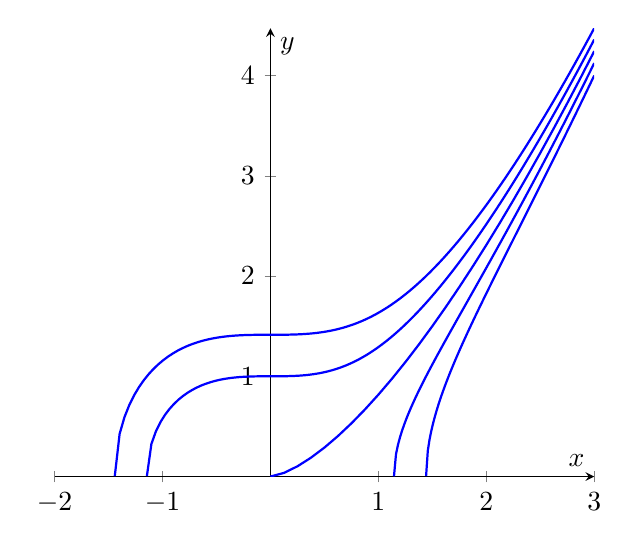
\begin{tikzpicture}
		\begin{axis}[axis lines = center, xmin = -2, xmax = 3, 
		xlabel = $x$, ylabel = $y$]
                \addplot[blue, thick, domain = 1.44226:3, samples = 100]
                {sqrt((2/3)*x^3 - 2)};
                \addplot[blue, thick, domain = 1.14472:3, samples = 100]
                {sqrt((2/3)*x^3 - 1)};
                \addplot[blue, thick, domain = 0:3]{sqrt((2/3)*x^3)};
                \addplot[blue, thick, domain = -1.14471:3, samples = 100]
                {sqrt((2/3)*x^3 + 1)};
                \addplot[blue, thick, domain = -1.44225:3, samples = 100]
                {sqrt((2/3)*x^3 + 2)};
            \end{axis}
	\end{tikzpicture}
    \caption{Several possible solutions to $\frac{dy}{dx} = 
    \frac{x^2}{y}$}
    \label{fig:solutions}
\end{figure}

It is not always possible to solve for $y$ explicitly in terms of 
$x$. The practice problem below is an example of this. 

\begin{Exercise}[label = diffeq1]
	Solve the differential equation $\frac{dy}{dx} = \frac{3x^2}{2y + \sin{y}}$. 
\end{Exercise}

\begin{Answer}[ref = diffeq1]
	$$\frac{dy}{dx} dx = \frac{3x^2}{2y + \sin{y}} dx$$
	$$(2y + \sin{y})(dy) = \frac{3x^2}{2y + \sin{y}}(2y + \sin{y})(dx)$$
	$$(2y + \sin{y})dy = (3x^2)dx$$
	$$\int 2y\,dy + \int \sin{y}\,dy = \int 3x^2\,dx$$
	$$y^2 - \cos{y} = x^3 + C$$
\end{Answer}

\section{Partial Differential Equations}

Partial differential equations (PDEs), on the other hand, involve a
function of multiple independent variables and their partial
derivatives. An example of a PDE is the heat equation, a second-order
PDE:\index{partial differential equations} \index{PDEs}

\begin{equation}
\frac{\partial u}{\partial t} = \alpha \frac{\partial^2 u}{\partial x^2}
\end{equation}

In this equation, $u = u(x, t)$ is a function of the two independent
variables $x$ and $t$, $\frac{\partial u}{\partial t}$ is the first
partial derivative of $u$ with respect to $t$, and $\frac{\partial^2
  u}{\partial x^2}$ is the second partial derivative of $u$ with
respect to $x$.



